Dieses Kapitel beleuchtet dieser Arbeit zugrunde liegende Konzepte und Algorithmen. Zunächst wird das Prinzip der Epipolargeometrie beschrieben welches ein wichtiges mathematisches Modell für photogrammetrische Verfahren darstellt. Daraufhin folgt eine Erläuterung des Terms \emph{Stereo Matching} sowie eine Klassifizierung in lokale und globale Algorithmen. Im Anschluss daran wird das Prinzip des \emph{Block Matching} Algorithmus beschrieben, welcher die Grundlage für den im Rahmen dieser Arbeit verwendeten \emph{Semi Global Block Matching} Algorithmus bildet. Anschließend erfolgt eine Erläuterung des im Rahmen dieser Arbeit entwickelten Frameworks sowie Details zur Implementierung dessen.

% ---------------------- section -----------------------
\section{Epipolargeometrie}
\label{sec:epipolargeometrie}
Photogrammetrische Verfahren nutzen oft das Konzept der Epipolargeometrie. Dieses mathematische Modell beschreibt die geometrische Beziehung zwischen verschiedenen Kamerabildern desselben Objektes, sowie die Beziehung korrespondierender Bildpunkte. Generell gesehen ist die der Epipolargeometrie zugrundeliegende Kamera durch das Lochkamera-Modell beschrieben. Dabei befindet sich jeder dreidimensionale Punkt des aufgenommenen Objektes mit dem Projektionszentrum sowie dem entsprechenden Bildpunkt auf einer Geraden.Unter Zuhilfenahme der räumlichen Orientierung, sowie der intrinisischen Parameter der Kamera (beispielsweise die Brennweite, Koordinaten des Bildhauptpunktes) ist es möglich den Schnittpunkt mehrere solcher Raumgeraden zu berechnen um die dreidimensionalen Koordinaten des Objektpunktes zu erhalten. Dabei gilt generell: wenn ein Punkt $P$ im linken Bild gegeben ist, so wird die Suche des korrespondierenden Punktes $P’$ auf die Epipolarlinie des rechten Bildes reduziert. Die algebraische Repräsentation der relativen Orientierung zweier Bilder ist die Fundamentalmatrix $F$. 

% GRAFIK: epipolargeometrie
\begin{figure}[h]
	\begin{center}
		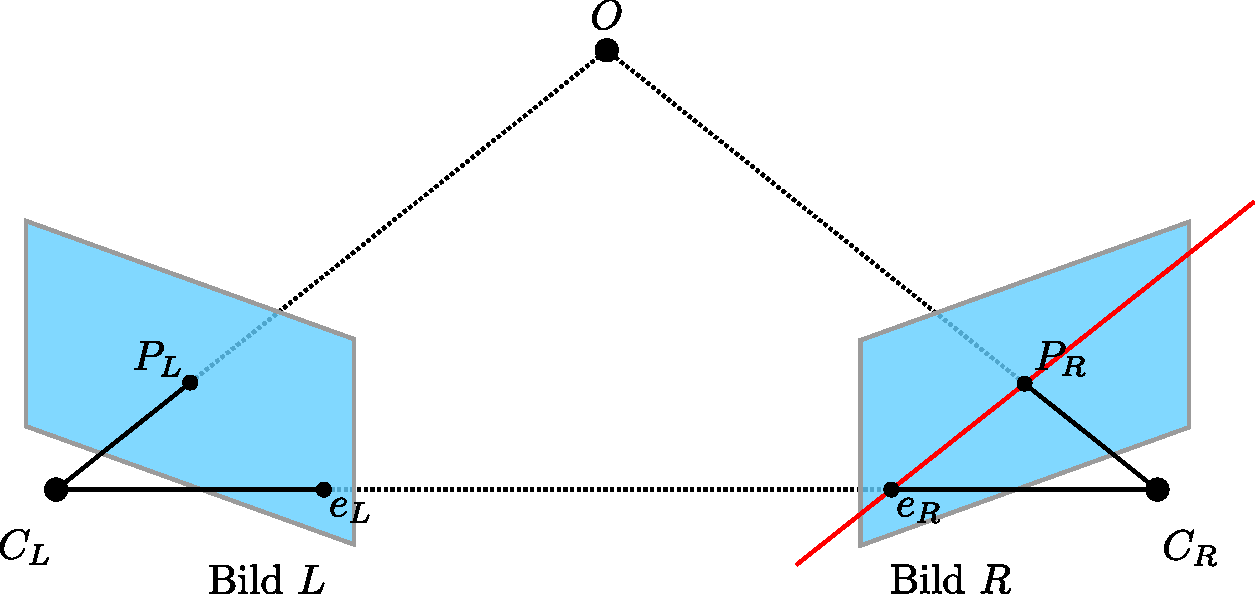
\includegraphics[width=10cm]{img/epipolar_geometry.pdf}
	\end{center}
	\caption{Darstellung der Epipolargeometrie.}
	\label{fig:epipolar_geometry}
\end{figure}

\noindent
Abbildung \ref{fig:epipolar_geometry} visualisiert diesen Prozess. Gegeben sind die beiden Projektionszentren $C_L$ und $C_R$ zweier Kameras, sowie die Bildpunkte $P_L$ und $P_R$, welche beide die Position des Objektpunktes $O$ in beiden Bilden beschreiben. Mit der Information über $C_L$ und $P_L$ allein kann keine Information über die räumliche Tiefe des Objektpunkts O abgeleitet werden. Die Projektion aller möglichen Positionen von O entlang des Raumstrahls in das rechte Bild ergibt eine Linie, die so genannte Epipolarlinie. Rechnerisch ergibt sich diese aus der Multiplikation des Bildpunktes mit der Fundamentalmatrix. Betrachtet man den Strahl $C_L,O$ aus Perspektive des rechten Bildes, und verschiebt $O$ entlang dessen, so ergibt sich die Epipolarlinie in $R$. Somit ist es möglich die Epipolarlinie $e_l,P_{x_2,y_2}$ zu bestimmten. Anhand dieser kann der Suchraum für den gesuchten korrespondierenden Bildpunkt im Rechten Bild auf die Epipolarlinie eingegrenzt werden. Kann der der gesuchte korrespondierende Punkt $P_R$ mittels eines \emph{Matching}-Ansatzes gefunden werden, ist es möglich die 3D Position des Objektpunktes zu triangulieren.\\

\noindent
Die Epipole sind durch den Schnittpunkt der Basislinie mit den beiden Bildebenen definiert. Im Falle des so genannten Stereonormalfalles ist ein Schnittpunkt der Basislinie mit den Bildebenen nicht möglich, da die Epipole in der Unendlichkeit und parallel zur x-Achse liegen. Da in diesem Fall die Bildebenen in einer Ebene liegen und die Blickrichtungen und Koordinatenachsen der Kamerassysteme parallel ausgerichtet sind, sind alle Epipolarlinien parallel. Des Weiteren beschränkt sich die Suche nach einem korrespondierenden Punkt $(x_L, y_L)$ auf eine Suche entlang der horizontalen Epipolarlinie mit konstander y-Koordinate $(y_R=y_L)$.


\section{Kamerakalibrierung und Rektifizierung}
\label{sec:camera_calibration}
Um den Prozess der Korrespondenzanalyse zu vereinfachen sind drei verschiedene Schritte nötig:
\begin{enumerate}
	\item Kalibrierung des Stereo-Kamerasystems
	\item Transformation der Bilder zum Stereonormalfall
	\item Rektifizierung der Bilder
\end{enumerate}
 Zunächst müssen die intrinsischen und extrinsischen Parameter des Stereo-Kamerasystems berechnet werden. Die Ermittlung der intrinischen Parameter ist dabei der Hauptbestandteil der Kalibrierung. Mit Hilfe weiterer Schritte kann auch die relative Orientierung der beiden Kameras des Systems ermittelt werden. Zu Beginn des Kalibrier-Prozesses werden Bilder eines Kalibrierobjektes aufgenommen. Dies ist meistens ein einfaches Schachbrettmuster mit ungleicher Anzahl an Quadraten, oder auch ein radiales Objekte mit einem spezifischerem Aufbau. Die Dimensionen des Kalibrierobjektes sind dabei bekannt. Der Prozess der Kalibierung zielt darauf ab die \enquote{inneren} Parameter der Kamera zu bestimmen. Dies beinhaltet einerseits die Kameramatrix in welcher Parameter wie die \emph{Principal Distance} (Abstand vom Projektionszentrum zur Bildebene), der Bildhauptpunkt (Principal Point) sowie das Seitenverhältnis der Pixel und der Scherungswinkel der Kamera. Weiterhin werden geometrische Verzerrungen des Bildes, beispielsweise Radiale Verzeichnungen durch die verwendete Optik, parametrisiert und somit nutzbar für die Entzerrung der Bilder in weiteren Schritten. Zudem werden bei der Kalibrierung die extrinsischen (äußeren) Parameter, d.h. die relative Orientierung der beiden Kameras zueinander, bestimmt. Zu diesen zählt die Translation (x, y und z) sowie die Rotation der Kamera um die jeweiligen Achsen des Weltkoordinatensystems (ausgedrückt durch drei Winkel). Ein spezieller Aspekt bei der Kalibierung von Stereo-Systemen ist die Berechnung der extrinsischen Parameter von einer Kamera zur anderen. Die dabei berechnete Translation einer Kamera zur Referenzkamera wird als Basislinie bezeichnet. Häufig ist die linke Kamera dabei die Referenzkamera. Die Kenntnis über die relative Orientierung von Stereo-Kameras führt dazu, dass man identifizierte korrespondierende Punkte in den Bildpaaren direkt metrisch triangulieren kann. Der Prozess der Parameterfindung ist in der Regel ein Prozess welcher einmalig nach dem Aufbau ausgeführt werden muss und solange währt, wie sich nichts am Aufbau der Kameras ändert (Optik, Translation, Rotation). Anschliessend werden die Bilder mithilfe der erhaltenen Parameter entzerrt.\\

\noindent
Folgend aus der Kalibrierung der Kameras beginnt der Prozess der Rektifizierung der Bilder. Dieser kann dabei in zwei Schritte unterteilt werden, zunächst die geometrische Enzerrung der Bilder, anschliessend die Berechnung der \emph{region of interest} (ROI) (der in beiden Bildern maximale sichtbare Bereich, sodass der gesamte Bildbereich gefült ist (siehe Abbildung \ref{fig:rectification} (b))) beider Bilder. Mithilfe der zuvor berechneten intrinsischen und extrinsischen Parameter kann nun die Transformation der beiden Kamerabilder in den Stereo-Normalfall erfolgen. Die Rotationen, die bewirken, dass die Epipole auf der x-Achse liegen, werden auf die Bilder angewendet, sodass die Epipole beider Bilder auf der x-Achse liegen. Nach Verschiebung der Epipole entlang der x-Achse ins Unendliche ist Parallelität der Epipolarlinien gewährleistet. Daraus resultieren parallele und orthogonale Blickrichtungen zur identischen Bildebene, somit sind beide Bildebenen Element derselben Ebene. Die finale ROI ergibt sich aus der Konjuktion der einzelnen ROIs. Nach der Rektifizierung, der geometrischen Entzerrung und dem Anwenden der ROIs auf beiden Kamerabildern entspricht die jeweilige Pixelreihe im linken Bild der Pixelreihe mit dem selben Index im rechten Bild. Abbildung \ref{fig:rectification} verdeutlicht den Ablauf der Rektifizierung, so ist in Abbildung \ref{fig:rectification} (c) erkennbar das sich die korrespondierenden Bildpunkte auf einer Epipolarlinie befinden.\\

\begin{figure}[!h]
	\centering
	\begin{tabular}{c}
	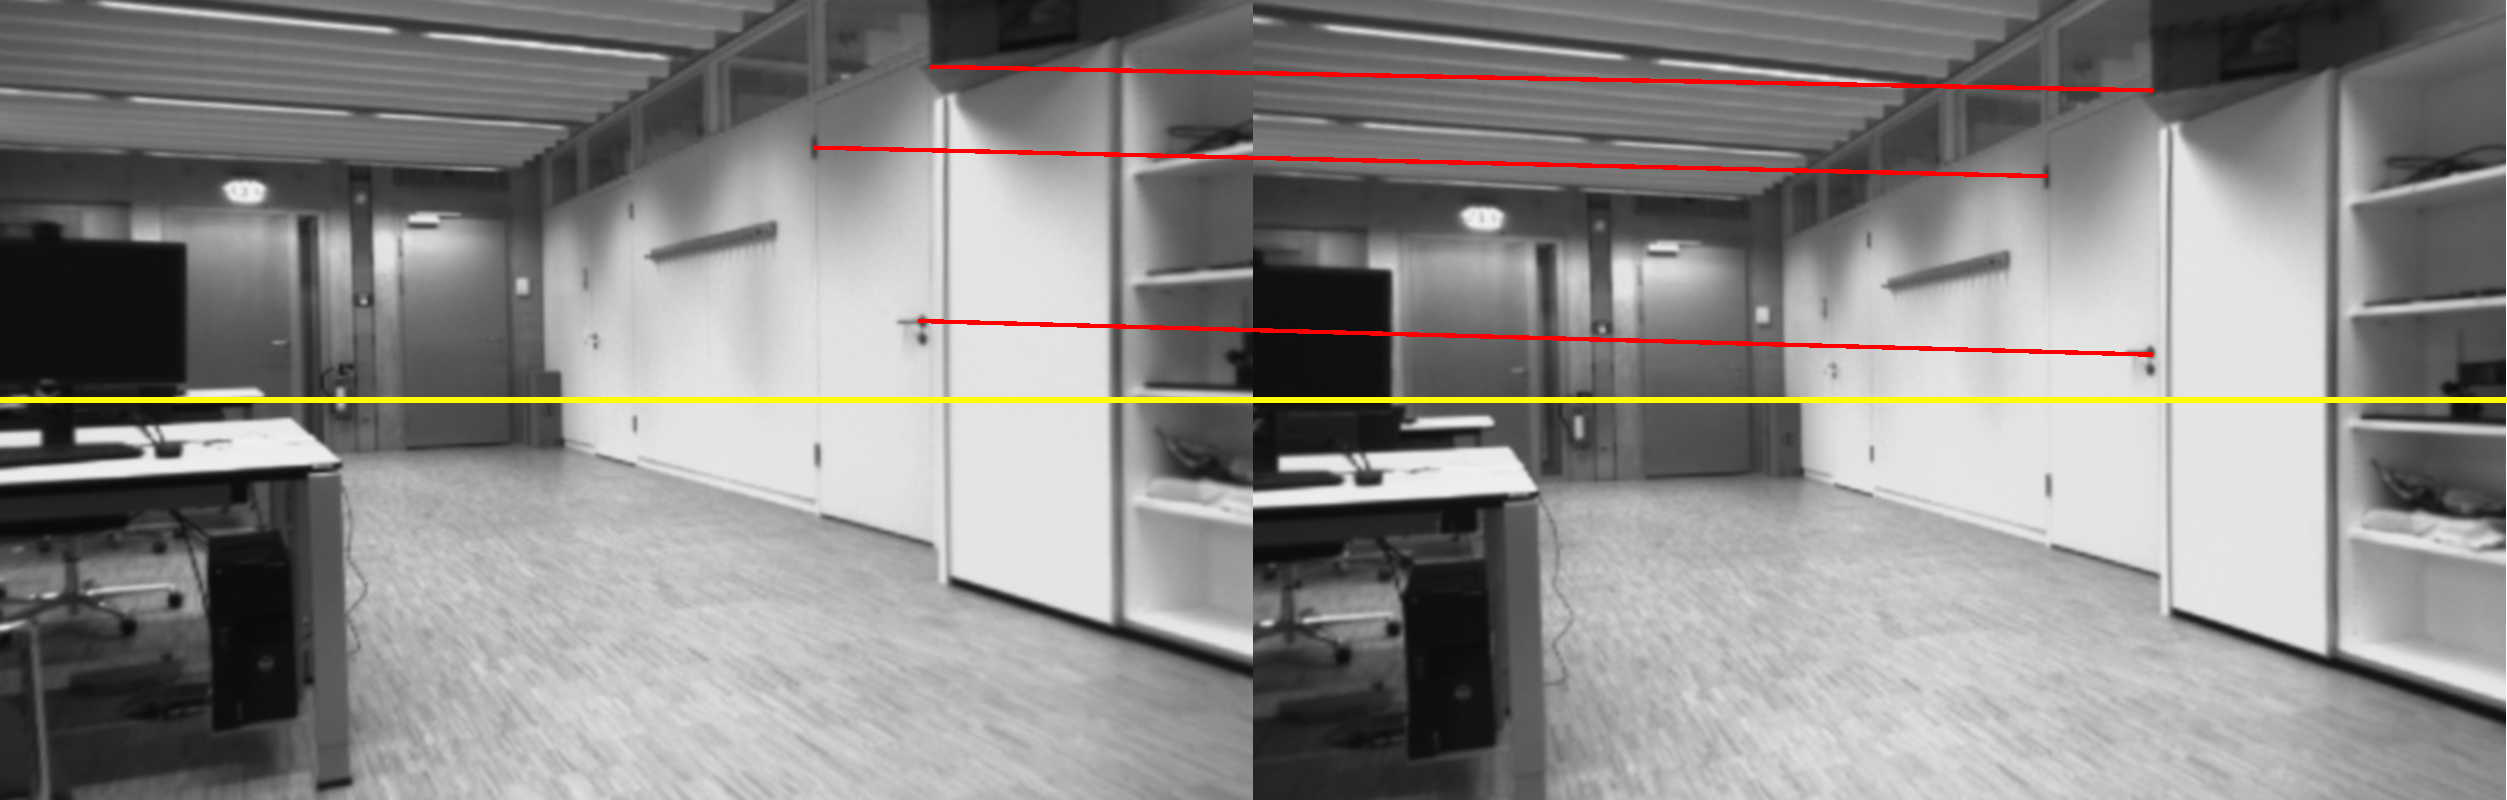
\includegraphics[width=10cm]{img/calibration/undistort}\\
	\small (a) Korrespondierende Punkte innerhalb der entzerrten Bilder.\\\\
	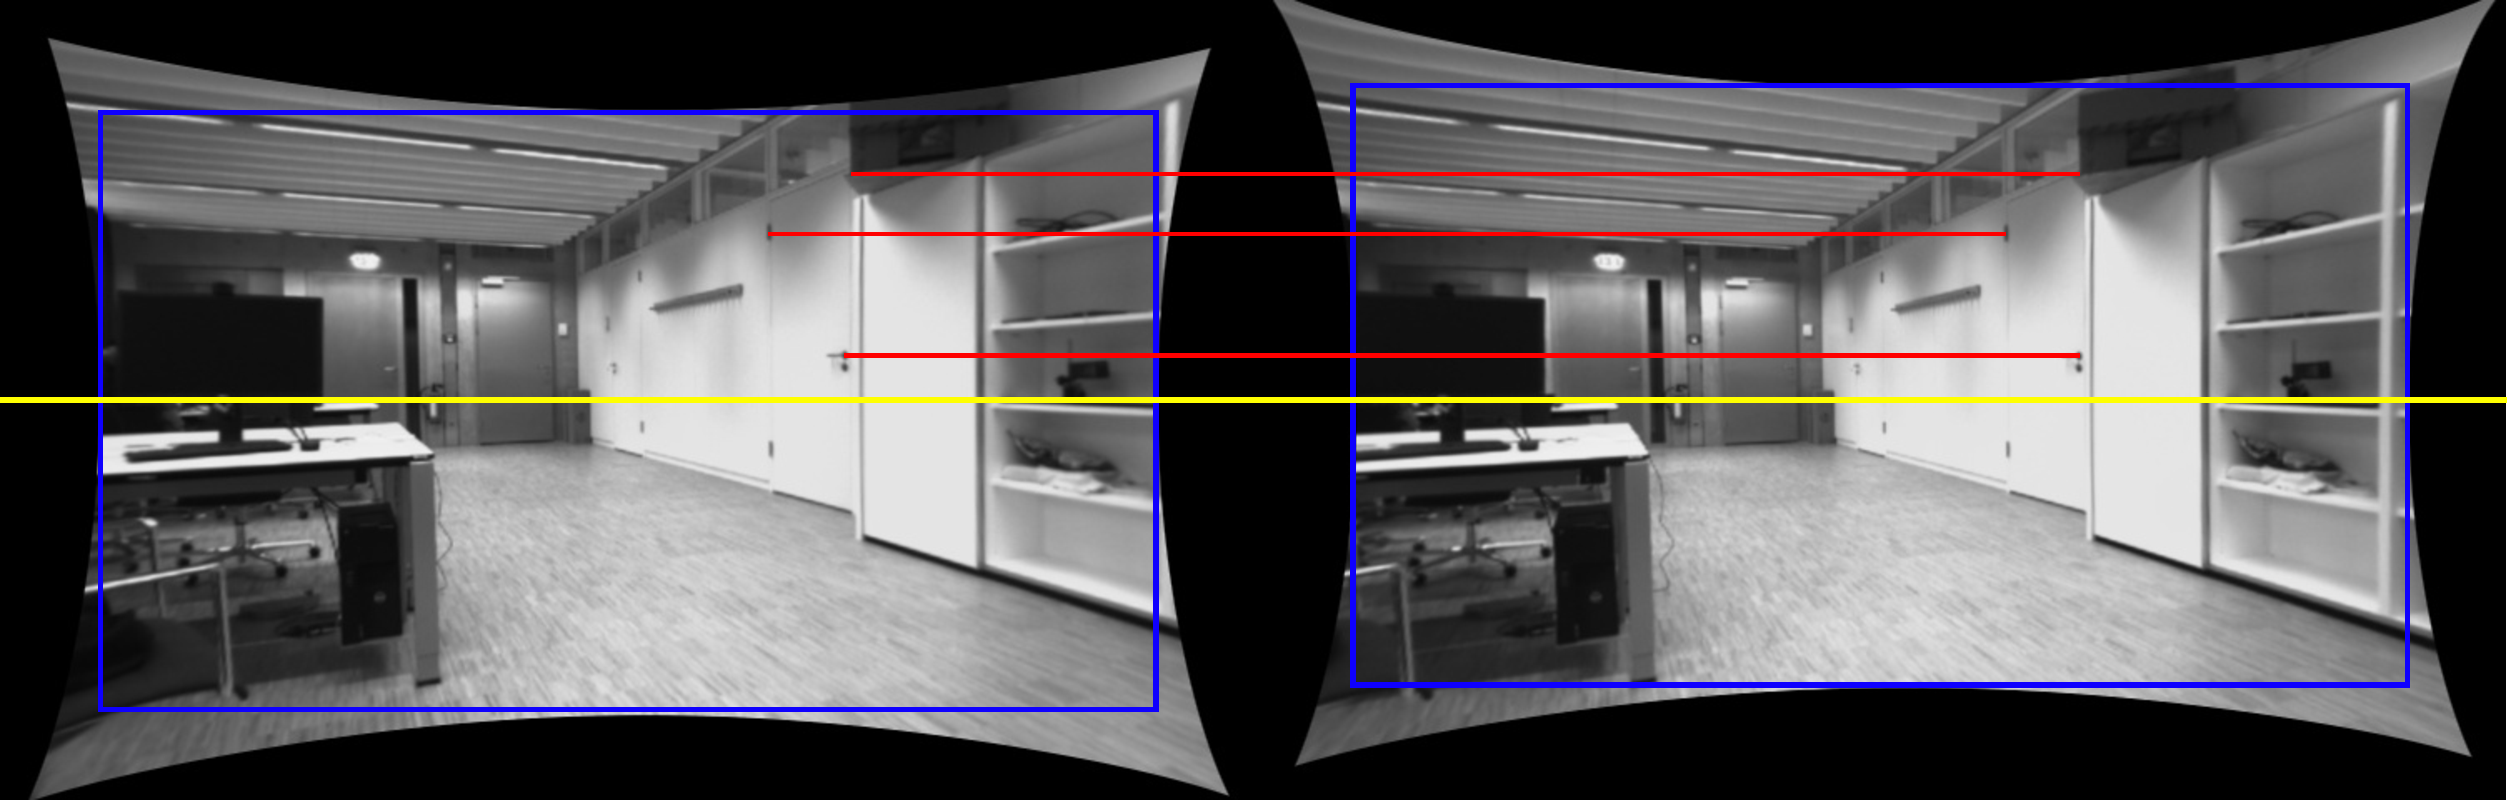
\includegraphics[width=10cm]{img/calibration/rect_uncropped.pdf}\\
	\small (b) Korrespondierende Punkte in den stereo-rektifizierten\\ und geometrisch entzerrten Bildern. Die ROIs (blau)\\ kennzeichnen die jeweils maximal möglichen\\ rechteckigen Flächen.\\\\
	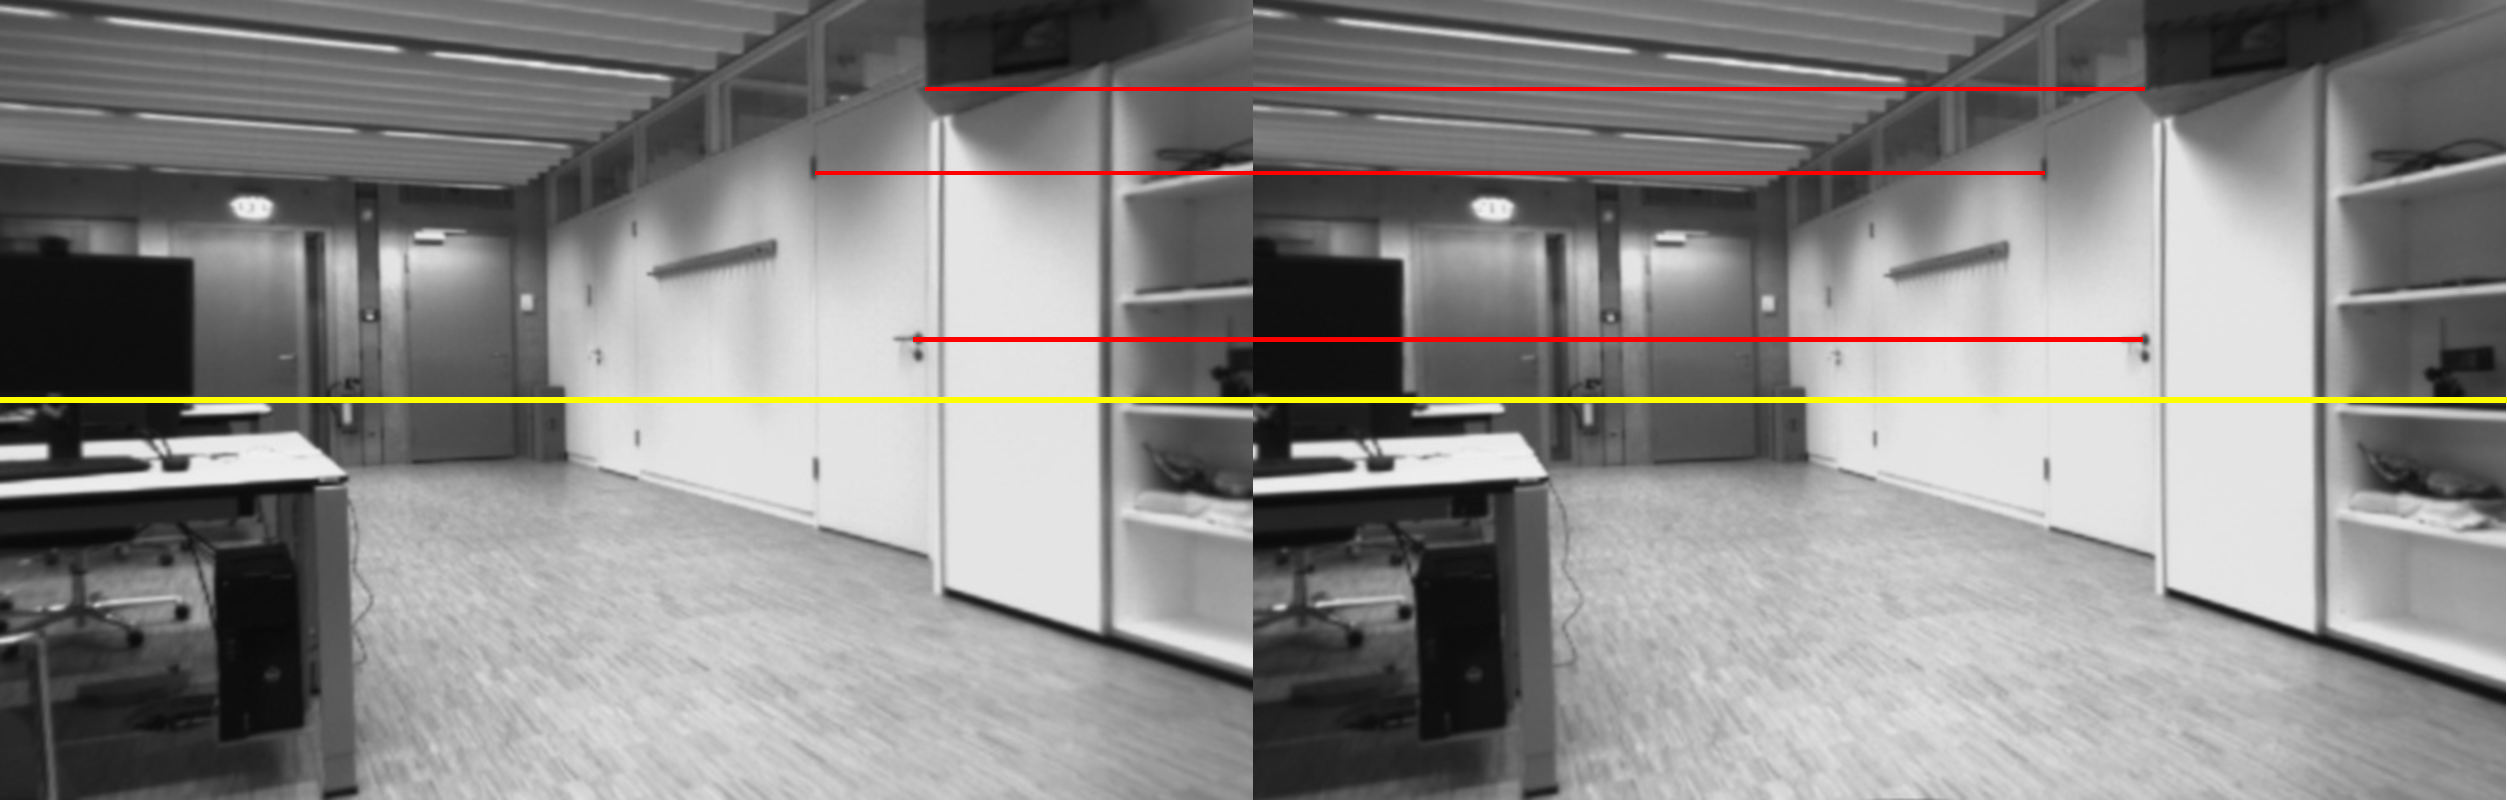
\includegraphics[width=10cm]{img/calibration/rect_cropped.pdf}\\
	\small (c) Korrespondierende Punkte in den beschnittenen, skalierten\\ und rektifizierten Bildern. \\\\
	\end{tabular}
\caption{Veranschaulichung des Effekts der Rektifizierung}
\label{fig:rectification}
\end{figure}

% ---------------------- section -----------------------
\section{Stereo Matching}
\label{sec:stereo_matching}
Mittels \emph{Stereo Matching} Verfahren wird versucht, für jeden Pixel in einem Bild der korrespondierende Punkt in einem zweiten Bild zu finden. Im Stereonormalfall ist die relative Orientierung der beiden Kameras bekannt und konstant. Des Weiteren werden korrespondierende Punkte in diesem Fall als einfache Differenz der x-Koordinaten, so genannte Disparitäten, dargestellt und gespeichert. Mithilfe der verschiedenen Perspektiven können Disparitäten zwischen korrespondierenden Pixeln berechnet werden. Die räumlichen 3D-Koorinaten der aufgenommenen Szene stehen im direkten (funktionalen) Zusammenhang mit der Information über die Disparität, der  relativen Orientierung der Kameras sowie der Kamerakalibrierung. Durch die Transformation zum Stereonormalfall vereinfacht sich dieser Zusammenhang enorm. Im Laufe des \emph{Stereo Matching} Prozesses kommt es zu zwei wesentlichen Problemstellungen: die Berechnung der Disparität (Stereo Korrespondenz) sowie die Invertierung der projektiven Geometrie, um dreidimensionale Informationen aus der errechnetet Disparität zu erhalten. Sofern eine Lösung beider Probleme vorhanden ist, können diese Informationen durch einfache Triangulierung errechnet werden.

\subsection{Lokale Methoden}
\label{subsec:local_methods}
Zur Berechnung der Disparität in lokalen \emph{Stereo Matching} Algorithmen gilt grundlegendes Prinzip: \enquote{Finde Pixel $P_2$ korrespondierend zu $P_1$ im Referenzbild}. Dabei wird die Korrelation von $P_1$ und $P_2$ unter Einbezug der lokalen Nachbarschaft bestimmt und die maximale Korrelation als Indikator für die Übereinstimmung von Pixeln herangezogen. Für die Korrelation wird jeweils die Bildinformation aus der lokalen Nachbarschaft um die zu testenden Pixel herangezogen, beispielsweise $11\times11$ Pixel. Geläufige Methoden dafür sind \emph{Sum of Absolute Differences} (SAD) (Hirschmüller 2011), \emph{Zero-mean Normalized Cross-Correlation} (ZNCC) (Chen \& Medioni, 1999), (Sára, 2002), \emph{Sum of Squared Differences} (SSD) (Cox et al., 1996). Jedoch können aufgrund des recht einfachen Ansatzes, der bei starken perspektivischen Änderungen und untexturierten Bereichen keine sinnvollen Ergebnisse liefert, falsche Berechnungen der räumlichen Tiefe auftreten, da benachbarte Pixel verschiedene Disparitäten aufweisen können (beispielsweise an horizontalen Kanten wie Türrahmen etc.). Strukturell gesehen sind lokale Methoden einfacher gehalten als globale Methoden, wodurch ein hoher Grad an Optimierung in der Implementierung möglich ist.

\subsubsection{Block Matching}
\label{subsec:stereo_matching_bm}
Einen der einfachsten Ansätze zur Berechnung von Korrespondenz zwischen zwei Bildern bietet der \emph{Block Matching} Algorithmus. Bei dieser lokalen Methode werden Blöcke bestimmter Größe mithilfe von Korrelation (Vergleich zweier Signale auf Übereinstimmung) auf Korrespondenz untersucht. Dabei reduziert die Epipolargeometrie diesen Prozess auf ein eindimensionales Problem, so dass ein Block im linken Bild mit allen potentiell möglichen Blöcken auf der Epipolarlinie des rechten Bildes verglichen wird. Das eigentliche Matching erfolgt über die Berechnung des gewählten Korrelationswerts eines Blockes mithilfe einer Energiefunktion.

\begin{figure}[h]
	\begin{center}
		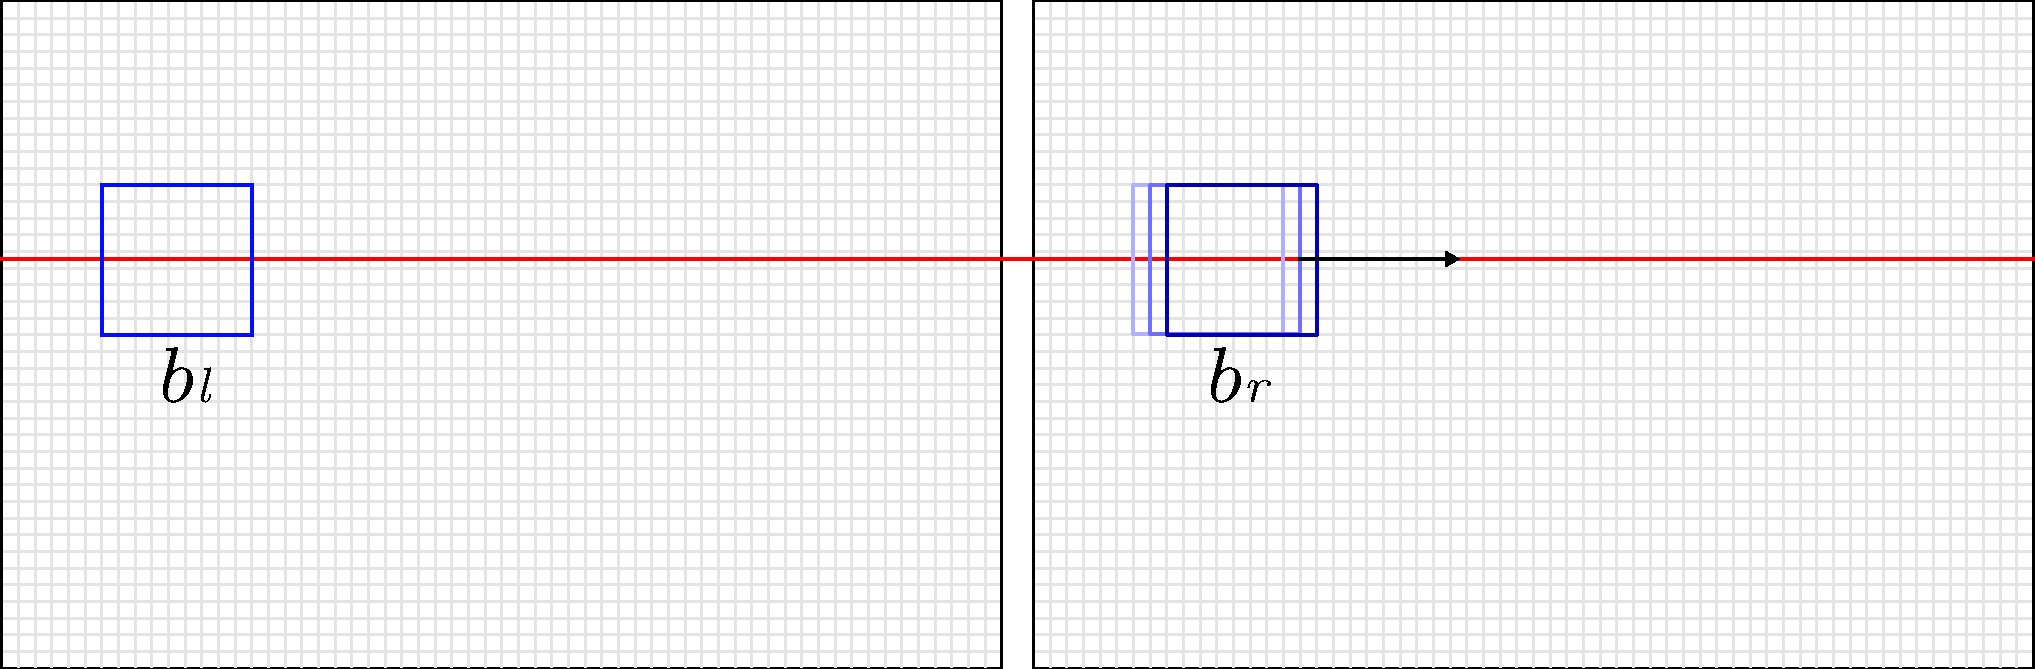
\includegraphics[width=13.5cm]{img/block_matching.pdf}
	\end{center}
	\caption{Visualisierung des Block Matching Algorithmus}
	\label{fig:block_matching}
\end{figure}

\noindent
Diesen Prozess veranschaulicht Abbildung \ref{fig:block_matching} . Durch den Fokus auf einzelne Pixelreihen und deren unmittelbare Umgebung ist dieses Verfahren wesentlich schneller, aber auch ungenauer als globale Matching Algorithmen. 


\subsection{Globale Methoden:}
\label{subsec:global_methods}
Bei globalen \emph{Stereo Matching} Algorithmen wird eine globale Annahme der zu betrachtenden Szene erstellt sowie eine ebenfalls globale Kostenfunktion definiert, welche es zu minimieren gilt. Dabei werden im Gegensatz zu lokalen Methoden die Korrespondenzen in einer Pixelreihe und die des gesamten Bildes miteinander verglichen. Zur Vereinfachung dieses Vorgangs betrachten einige Algorithmen nur die durch die Epipolargeometrie vorgegebenen Bildbereiche, wodurch ein zweidimensionales Problem auf ein eindimensionales reduziert wird. Resultierend daraus liegt die Stärke globaler Methoden in der Bewältigung schwacher Texturen sowie auftretender Okklusionen und unterschiedlicher Lichteinfälle, was, aufgrund der höheren Komplexität in einem höheren Rechen- und Speicheraufwand mündet. Weitere Verbesserungen der Ergebnisse können durch Techniken wie Dynamische Programmierung und \emph{Graph Cut} erreicht werden (\cite{zureiki2008stereo}).


\subsubsection{Semi Global Block M1atching}
\label{subsec:stereo_matching_sgbm}
Das im Rahmen dieser Arbeit verwendete Verfahren zur Berechnung von Disparitätenkarten ist der in der freien Computer Vision Bibliothek OpenCV \cite{opencv} implementierte \emph{Semi Global Block Matching} Algorithmus. Diese leicht abgewandelte Implementierung des \emph{Semi Global Matching} (SGM) Algorithmus von Hirschmüller et. al \cite{hirschmuller2005sgm} zeichnet sich sowohl durch seine guten Ergebnisse, als auch durch seine performante Berechnung aus. Durch die Verwendung von Blöcken anstelle einzelner Pixel ist dieser zu Teilen den Globalen Methoden zuzuordnen. Unter Zuhilfenahme dieses Verfahren ist es möglich, Disparitätenkarten in Echtzeit zu berechnen. Im Folgenden wird zunächst die grundlegende Funktionsweise des SGM erläutert. Im Anschluss daran werden die Unterschiede zum SGBM herausgearbeitet sowie eine kurze Erklärung der wesentlichsten Parameter dessen vorgenommen.\\

\noindent
\textbf{SGM:} \\
Die grundlegende Idee des \emph{Semi-Global Matching} Algorithmus besteht in dem pixelweisen Matching mittels \emph{Mutual Information} \footnote{\emph{Mutual Information}(MI), zu deutsch Transinformationen, beschreiben den statistischen Zusammenhang zweier Zufallsgrößen. Genauer gesagt beschreiben sie die Höhe des Informationsgehaltes einer Zufallsvariable aus anderen zufällig gewählten Werten.}. Ausgangsvorraussetzung dafür sind verschiedene Bilder derselben Szene mit vorhandener und bekannter Epipolargeometrie. Ein weiteres Kernelement des SGM ist die Anwendung eines globalen zweidimensionalen Glattheitskriteriums, was durch die Kombination mehrerer eindimensionaler Beschränkungen approximiert wird. Zunächst werden für jeden Pixel $P$ aus der Intensität $I_{bp}$ sowie der vermuteten Korrespondenz $I_{mq}$ auf der Epipolarlinie $q=e_{bm}(pd)$ die Matching Kosten berechnet. Zur Berechnung der MI wird zunächst eine initiale Disparitätenkarte benötigt. Diese wird nach dem Ansatz von Kim et al. \cite{kim2003visual} zufällig gewählt, um die Kosten berechnen zu können. Zur Steigerung der Performance wird die Disparitätenkarte zunächst nur mit halber Auflösung berechnet, wodurch der Rechenaufwand um den Faktor $8$ reduziert wird. Zur Vermeidung falscher Kostenberechnungen durch auftretendes Rauschen innerhalb des Bildes werden benachbarte Disparitäten mit in die Berechnungen einbezogen.\\

\noindent
Das letzte Problem besteht in der Berechnung der Korrespondenz sowie der daraus resultierenden Disparitäten. Dabei wird nach der Disparität $D$ mit der geringsten berechneten Energiefunktion gesucht. Anstatt nun einfach den minimalsten Pfad der Kosten zu summieren, werden zusätzlich auch andere Richtungen zur aktuellen Disparität mit einbezogen (siehe Abbildung \ref{fig:sgm_directions}).

\begin{figure}[h]
	\centering
	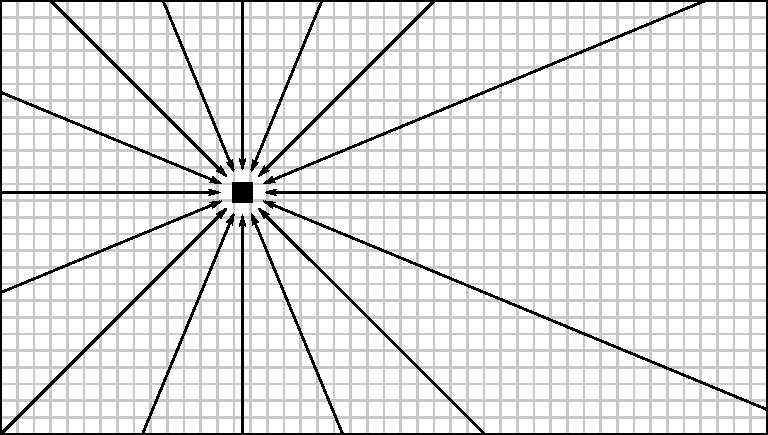
\includegraphics[width=12cm]{img/sgm_directions.pdf}
	\caption{Darstellung der verschiedenen betrachtetend Richtungen des SGBM}
	\label{fig:sgm_directions}
\end{figure}

\noindent
Um das 2D-Glattheitskriterium möglichst gut zu approximieren,  sollten dabei mindestens 8 Richtungen vorliegen, eine vermehrte Anzahl an Richtungen, etwa 16, ist dabei vorteilhaft. Die berechnete Disparität ergibt sich aus den minimalen Kosten anhand dieser Pfade.\\

\noindent
\textbf{SGBM:} \\
Der \emph{Semi Global Block Matching} Algorithmus ist ein in der Computer Vision Library OpenCV implementiertes Verfahren zur schnellen Berechnung von Disparitätenkarten. Die Grundlage dafür bietet Hirschmüller et al.’s SGM \cite{hirschmueller2008sgm} mit den folgenden grundlegenden Änderungen:

\begin{enumerate}[label=C.\arabic*]
	\item Statt den originalen 8 bzw. 16 Richtungen werden nur 5 betrachtet. \label{item:differences_directions}
	\item Es werden  standartmäßig keine einzelnen Pixel sondern Blöcke verglichen. \label{item:differences_matching}
	\item Anstelle der \emph{Mutual Information} Kostenfunktion wird das von Birchfield et al. vorgestellte \emph{Sub-Pixel Dissimilarity Measurement} Verfahren verwendet \cite{birchfield-tomasi}.
	\item Verschiedene Schritte der Vor- und Nachprozessierung des \emph{StereoBM} Algorithmus werden verwendet, dazu zählen Filtermethoden wie quatdratische Interpolation oder Sprenkelfilter.
\end{enumerate}

\noindent
Dies ermöglicht eine schnelle Berechnung der Disparitäten auf einem qualitativ hochwertigen Niveau. Der geringe Verlust an Qualität, hervorgerufen durch die geringere Anzahl an betrachteten Richtungen, kann in Anbetracht der Berechnung in Echtzeit vernachlässigt werden.\\

\begin{figure}[h]
\centering
	\begin{tabular}{m{2cm} m{3.3cm} m{3.3cm} m{3.3cm}}
	{\scriptsize Datensatz}&
	\begin{center} {\scriptsize Tskukuba} \end{center} &
	\begin{center} {\scriptsize Teddy} \end{center} &
	\begin{center} {\scriptsize Cones} \end{center}
	\\
	{\scriptsize Bilder links} &
	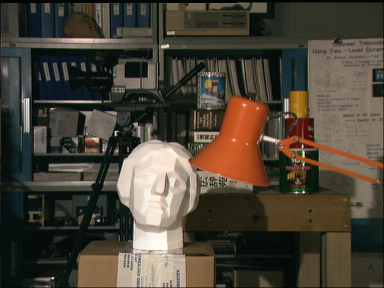
\includegraphics[width=3cm]{img/disparity_images/left_tsukuba.png} & 
	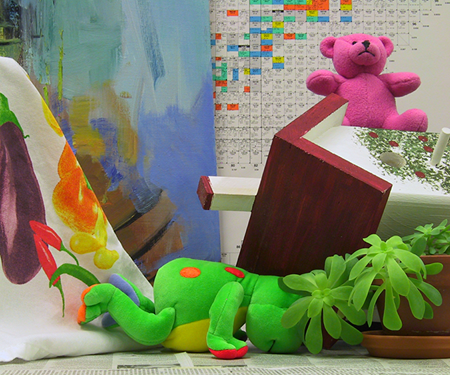
\includegraphics[width=3cm]{img/disparity_images/left_teddy.png} & 
	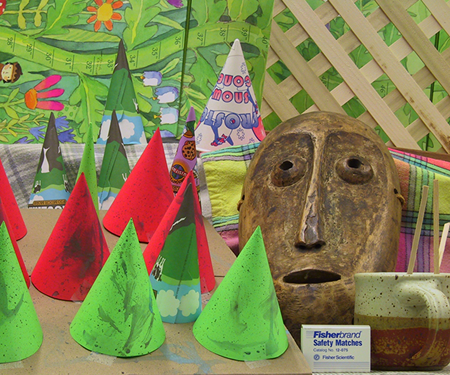
\includegraphics[width=3cm]{img/disparity_images/left_cones.png} 
	\\ 
	{\scriptsize Ground Truth} &
	
\includegraphics[width=3cm]{img/disparity_images/gt_tsukuba.png} & 
	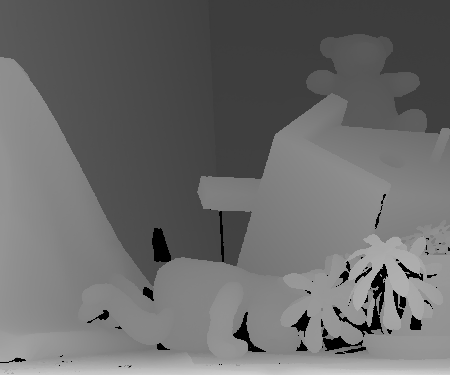
\includegraphics[width=3cm]{img/disparity_images/gt_teddy.png} & 
	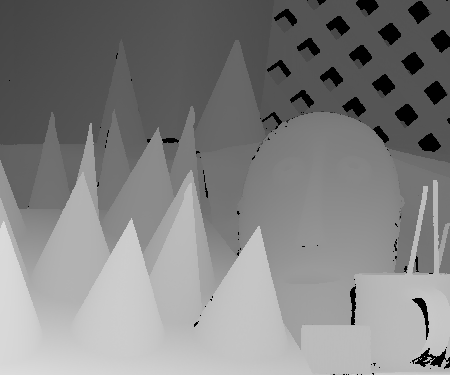
\includegraphics[width=3cm]{img/disparity_images/gt_cones.png} 
	\\
	{\scriptsize SGM (MI)} &
	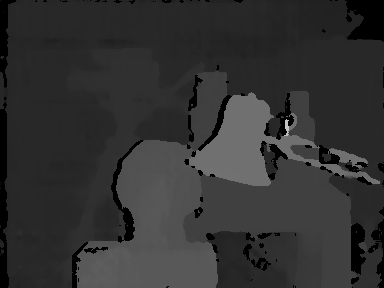
\includegraphics[width=3cm]{img/disparity_images/sgm_tsukuba.png} &
	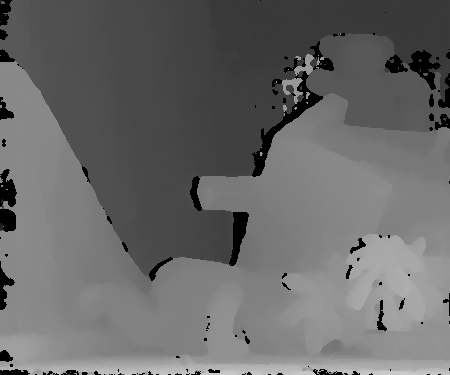
\includegraphics[width=3cm]{img/disparity_images/sgm_teddy.png} &
	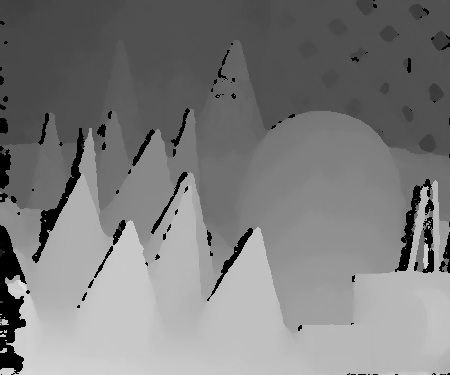
\includegraphics[width=3cm]{img/disparity_images/sgm_cones.png}
	\\ 
	{\scriptsize SGBM} &
	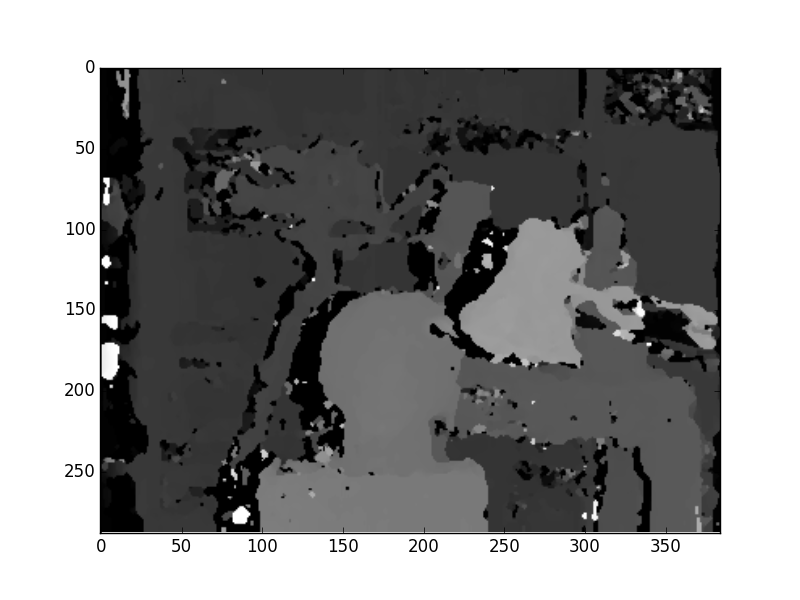
\includegraphics[width=3cm]{img/disparity_images/sgbm_tsukuba.png} &
	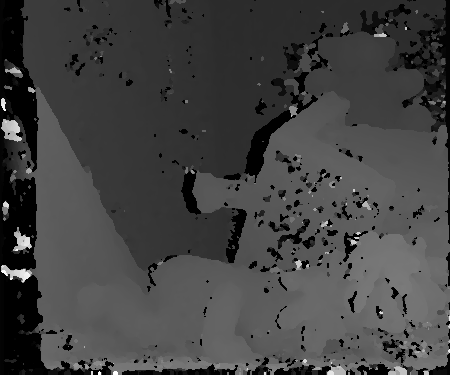
\includegraphics[width=3cm]{img/disparity_images/sgbm_teddy.png} &
	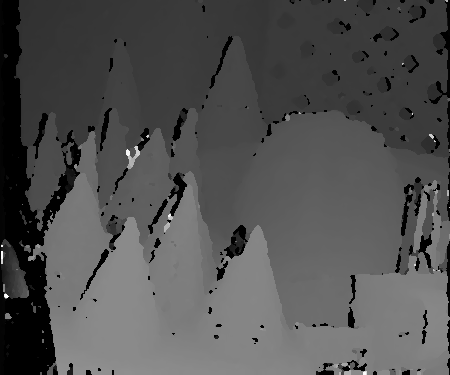
\includegraphics[width=3cm]{img/disparity_images/sgbm_cones.png}
	 \\ 
	\end{tabular}
\caption{Vergleich zwischen Ground Truth Bildern sowie dem SGM(2005) und OpenCV's SGBM}
\label{fig:disparity_comparison}
\end{figure}
% TODO vielleicht eigene Bilder verbessern, sodass tsukuba nicht ganz so crappy aussieht

\noindent
Abbildung \ref{fig:disparity_comparison} stellt die originalen Bilder der Szene (\cite{middlebury_data}), die mithilfe von strukturiertem Licht aufgenommenen \emph{Ground Truth} Bilder sowie die jeweiligen berechneten Tiefenkarten durch den SGM und den SGBM dar. Aus dieser ist der Qualitätsverlust des SGBM beim Tsukuba- sowie beim Teddy Datensatz zu erkennen.\\

\noindent
Trotz dessen sind die Grundformen sowie die berechnete Tiefe klar erkennbar. Grundlegend bietet der SGBM eine qualitativ hochwertige Berechnung von Tiefenkarten. Weiterhin ist die Berechnung sowie die daraus resultierenden Disparitätenkarten stabiler. Bei der Berechnung durch OpenCV's einfachen Block Matching Algorithmus kann es, in Abhängigkeit der zu rekonstruierenden Szene zu einem Flackern zwischen den einzelnen Einzelbildern kommen. Dies würde bedeuten das eventuell keine Informationen zwischen zwei Frames vorliegen was wiederum zu Fehlern in der Erkennung führen würde.\\

\noindent
Weiterhin existiert eine Reihe verschiedener Parameter welche die Berechnung der Disparity Map aktiv beeinflussen. Im folgenden werden die zur Initialisierung obligatorischen Parameter in ihrer Funktionsweise grob beschrieben.

\begin{itemize}
	\item \textbf{\emph{minDisparity:}}\\
	Der Parameter \emph{minDisparity} begrenzt den messbaren Tiefenbereich nach oben. Er beschreibt also die minimale zu erkennende Disparität und somit die maximale zu erkennende Distanz.
 	\item \textbf{\emph{numDisparities:}}\\
 	Mit Hilfe der \emph{Number of Disparities} \emph{numDisparities} wird die Breite des Matchingbereiches festgelegt. Geht man davon aus, dass das linke Bild Referenz ist, wird damit festgelegt, wie viele Pixel im rechten Bild auf Korrespondenz untersucht werden sollen. In Abhängigkeit der Größe beider Parameter können in der Tiefenkarte Bereiche entstehen, die keine sinnvolle Information enthalten. Die damit verbundene weitere Verfahrensweise wird im Abschnitt \ref{sec:preprocessing} näher erläutert.
	\item \textbf{\emph{blockSize:}}\\
	Die \emph{blockSize} des SGBM beschreibt die Größe des Matching Blocks in Pixeln. Je größer der Wert gewählt wird, desto weicher wird die resultierende Disparitätenkarte. Dabei gehen jedoch auch Detailinformationen, beispielsweise bezüglich feiner Strukturen in der Szene verloren. Ist der Wert niedrig so ist es unter Umständen schwerer homogene Flächen korrekt zu Matchen. Zudem können eventuell weniger Korrespondenzen gefunden werden.
\end{itemize}

% ---------------------- section -----------------------
\section{mvStereoVision Framework}
\label{sec:framework}
Das verwendete \emph{Framework} zur Bildaufnahme und Berechnung der Disparitätenkarten bedient sich der von Matrix Vision zur Verfügung gestellte Bibliothek \cite{matrixvision} zur Kommunikation mit den Kameras, sowie OpenCV \cite{opencv} zur Verarbeitung der Bilder. Die wesentlichen Funktionen werden im folgenden näher beleuchtet.\\

\noindent
\textbf{Bildaufnahme:}\\
Die Aufnahme der einzelnen Bilder beginnt bei einer Anfrage an die Kamera nach den jeweiligen Rohdaten. Diese werden nun an die \emph{Stereosystem} Klasse weitergegeben, in welcher die Bilder anschliessend mithilfe der durch die Kalibrierung ermittelten Parameter in den Stereonormalfall transformiert, geometrisch entzerrt und beschnitten werden. Damit ist der Abschnitt der Vorprozessierung abgeschlossen, an dessen Ende sich beide Bilder im \emph{Stereopair} Objekt befinden. Die Aufnahme der Bilder erfolgt dabei in separaten Threads um unabhängig von weiteren Berechnungen Bilder aufzunehmen. Anschliessend wird das \textit{Stereopair} Objekt an die Berechnung der Disparitätenkarte in einen separaten Thread übergeben. Sofern eine neue Tiefenkarte vorliegt wird innerhalb des Hauptprogramms mit Hilfe eines Wahrheitswertes darüber informiert. Der gesamte Prozess wird in Abbildung \ref{fig:framework_pipeline} visualisiert.\\
 
\begin{figure}[h]
	\begin{center}
		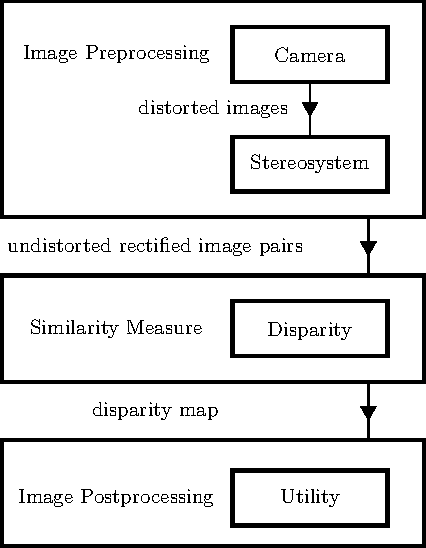
\includegraphics[width=6cm]{img/framework_pipeline.pdf}
	\end{center}
	\caption{Ablauf der Bildaufnahme, Berechnung der Disparitätekarte sowie weiteren Verarbeitung}
	\label{fig:framework_pipeline}
\end{figure}


\noindent
\textbf{Distanzberechnung:}\\
Für die Berechnung von 3D-Koordinaten auf der Basis von Bildkoordinaten sowie der inneren und relativen Orientierung des Stereo-Systems wird die Reprojektionsmatrix $Q$, welche im Rahmen der Rektifizierung berechnet wird benötigt. Diese ist wie folgt aufgebaut:
\begin{equation}
    Q= 
    \begin{bmatrix}
      1 & 0 & 0 & -C_x\\
      0 & 1 & 0 & -C_y\\
      0 & 0 & 0 & f\\
      0 & 0 & \frac{-1}{T_x} & \frac{C_x - C_x'}{T_x}
    \end{bmatrix}
    \longrightarrow
    \begin{bmatrix}
      1 & 0 & 0 & -C_x\\
      0 & 1 & 0 & -C_y\\
      0 & 0 & 0 & f\\
      0 & 0 & a & b
    \end{bmatrix}
\end{equation}
Dabei beschreiben $-C_x$ und $-C_y$ die beiden negativen Koordinaten des Bildhauptpunktes der Referenzkamera, beispielsweise der linken. Der Parameter $f$ beschreibt die Brennweite der linken Kamera. $T_x$ ist die horizontale Translation zwischen beiden Kameras. Die in der Q-Matrix enthaltenen Parameter sind mit Ausnahme von $C_x'$ alle die der linken Kamera. Es wird angenommen, dass es sich um einen (nach der Rektifizierung vorhandenen) Stereonormalfall handelt und sich die beiden Strahlen der Bildhauptpunkte in der Unendlichkeit schneiden. Dies führt zu einer Annäherung des unteren rechten Parameters in 2.1 an $0$. Zur einfacheren Darstellung und Erläuterung werden die Basislinie der Kamera $\frac{-1}{T_x}$ im folgenden als $a$ sowie die Darstellung beider Bildhauptpunkte $\frac{C_x - C_x'}{T_x}$ als $b$ notiert.\\

\noindent
Eine Eigenschaft der Reprojektionsmatrix ist die einfache Berechnung von dreidimensionalen Weltkoordinaten. Diese Berechnung erfolgt mittels Gleichung \ref{eq:distance_calculation}. Dabei beschreibt der Parameter $d(I_x,I_y)$ den Pixelwert der Disparitätenkarte an den Bildkoordinaten $I_x,I_y$.

\begin{equation}\label{eq:distance_calculation}
    \begin{aligned}
        \begin{bmatrix}
            X\\ Y \\ Z\\ W
        \end{bmatrix}
        = Q \cdot 
        \begin{bmatrix}
            I_x\\ I_y \\ d(I_x,I_y)\\ 1
        \end{bmatrix}\\
        3d\_coordinate = [\frac{X}{W}, \frac{Y}{W}, \frac{Z}{W} ]
    \end{aligned}
\end{equation}

\noindent
Die eigentliche Berechnung der einzelnen Parameter ergibt sich somit aus der Multiplikation des Vektors mit der Reprojektionsmatrix. Die dreidimensionalen Koordinaten ergeben sich damit aus:

\begin{equation}
  \begin{aligned}
        X &= I_x - C_x\\
        Y &= I_y - C_y\\
        Z &= f\\
        W &= d \cdot a + b
  \end{aligned}
\end{equation}